\chapter{Modelos de Análise}
% $<$Define any other requirements not covered elsewhere in the SRS. This might
% include database requirements, internationalization requirements, legal
% requirements, reuse objectives for the project, and so on. Add any new sections
% that are pertinent to the project.$>$

% \section{Appendix A: Glossary}
% %see https://en.wikibooks.org/wiki/LaTeX/Glossary
% $<$Define all the terms necessary to properly interpret the SRS, including
% acronyms and abbreviations. You may wish to build a separate glossary that spans
% multiple projects or the entire organization, and just include terms specific to
% a single project in each SRS.$>$

% \section{Apendice A: Modelos de Análise}
% $<$Optionally, include any pertinent analysis models, such as data flow
% diagrams, class diagrams, state-transition diagrams, or entity-relationship
% diagrams.$>$

\begin{center}
    \pagebreak

    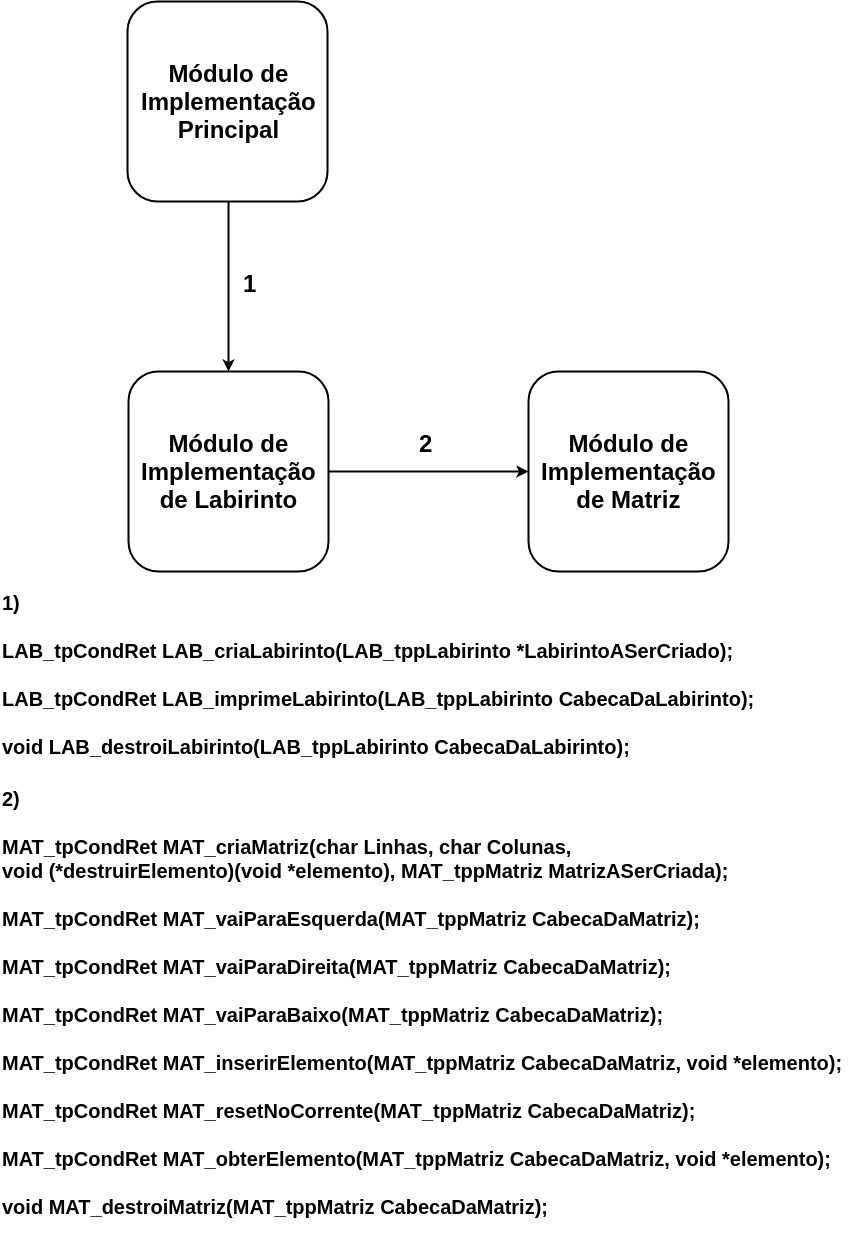
\includegraphics[width=1\textwidth]{arquitetura.png}
    
    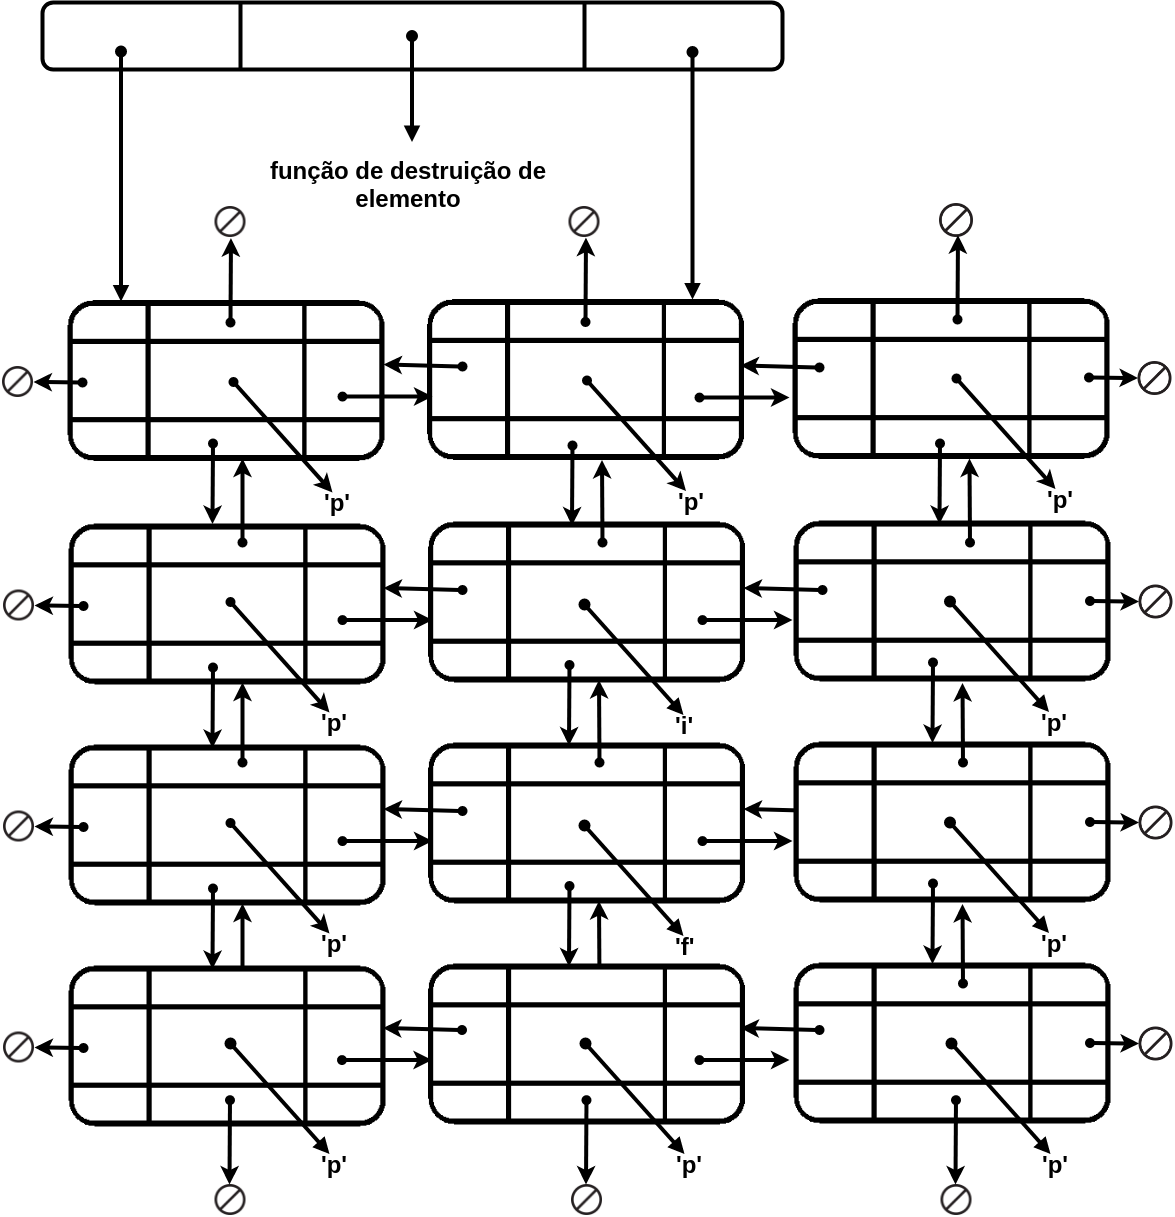
\includegraphics[width=1\textwidth]{exemplo.png}

    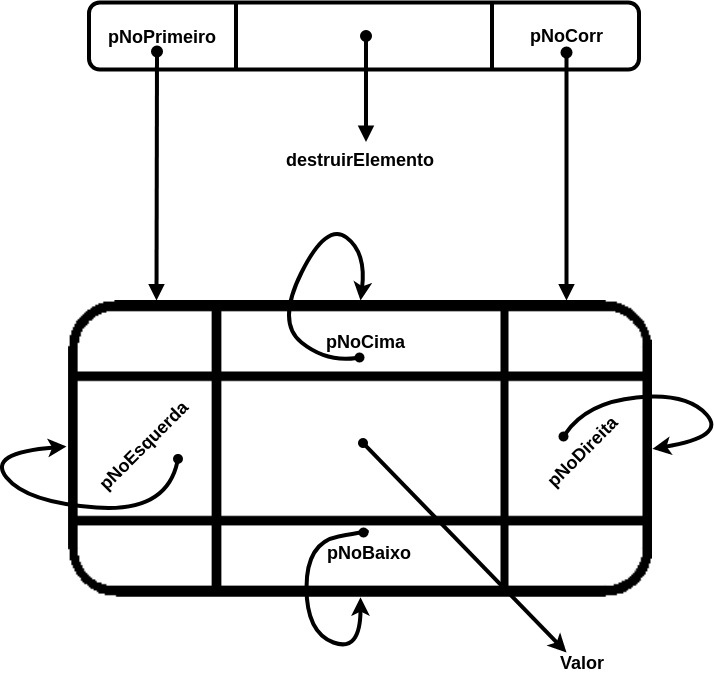
\includegraphics[width=1\textwidth]{modelofisico.png}
\end{center}

% \section{Appendix C: To Be Determined List}
% $<$Collect a numbered list of the TBD (to be determined) references that remain
% in the SRS so they can be tracked to closure.$>$
